\chapter{Neturon - Gamma Discrimination}
\label{ch:SecElectron}

Effective neutron-gamma discrimination is integral to the performance of the detector.
Generally, two methods are available for discrimination; 1) pulse shape discrimination and 2) pulse height discrimination.
In pulse shape discrimination the different decay times between the neutron and gamma pulses are exploited to develop a metric that allows for the classification of the pulse.
Generally, pulse shape discrimination works best when the pulses are noticeably different.
Pulse height discrimination is based on setting a pulse height discriminator that acts as a partition between two classes of pulses.
This is generally easier to implement than pulse shape discrimination.
While some of the fabricated films show a small basis for pulse shape discrimination, this work will only focus on pulse height discrimination.

The pulse height discriminator setting necessary to achieve the neutron-gamma discrimination is achieved through the use of a mathematical lower level discriminator (MLLD).
This virtual discriminator establishes the bound where $\epsilon_{int,\gamma n}\leq 10^{-6}$, and counts above the MLLD are classified as neutron counts. 

It is currently understood that the light output per path length of the film (which is directly proportional to the pulses collected on the PMT) is related to the stopping power of the radiation in the film material.
This is described by the Birks equation \eqref{eqn:BirksEquation}
\begin{align}
  \label{eqn:BirksEquation}
  \frac{dL}{dx} = \frac{S_B\frac{dE}{dx}}{1+kB\frac{dE}{dx}}
\end{align}
where \definevar{$S_B$}{absolute scintillation efficiency},\definevar{$\frac{dE}{dx}$}{linear stopping power} and \definevar{$kB$}{Birks parameter}.
For a given material the stopping power of the film will be constant, and therefore the light output of the film can be found by integrating the light output per path length over the total length of the film.
It is then possible to observe that the light output of a film is proportional to the energy deposited in the film.

\section{Charged Particle Interactions and Ranges}

The theoritical basis for the differnece in energy deposition lies in the differnet mechanisms between charged particle interactions and photon interactions in matter.
For photons with energies between approximately \SI{0.5}{\MeV} and \SI{5}{\MeV} Compton scattering is the prediomant interaction mechanism between the material and the photon.
The probability of an electron having a given kinetic energy after scattering can be expressed as \autoref{eqn:dSdEKlienNishina} (see \autoref{ch:ComptonScatter} for derivation details)
\begin{align}
  \label{eqn:dSdEKleinNishina}
\frac{d\sigma}{dE_e} = 2\pi r_e^2 \sin \theta f(\theta)\left [ \frac{1+\frac{E}{m_e c^2}\left(1-\cos\theta \right)^2}{E^2 \sin \theta} \right ]
\end{align}

It is proposed to optimize the neutron-gamma discrimination by focusing on the energy deposition in the film.
Preferential energy deposition by neutrons relative to gammas will enhance the discrimination by creating larger neutron light pulses than the gamma pulses, allowing for fewer neutron pulses to be classified as gamma pulses because they are below the MLLD.
The product of this work will be a measurement validated simulation capability for the energy deposition in polymeric films (focusing on polystyrene).
The simulation capability will be applied to the optimization of the polystyrene film system.

\subsection{Methodology}

The GEANT4 toolkit has the ability to track the energy deposition in different materials as well as the tracking of electrons to a least \SI{1}{\keV}\cite{agostinelli_geant4simulation_2003}.
It is proposed to represent the detector geometry as a single layer of neutron absorbing thin polymeric film mounted on top of a non-scintillating material (PMMA).
For simplicity, the initial events for runs will be chosen by setting up a particle gun for thermal (\SI{0.025}{\eV}) neutrons upon the detector and for both gammas resulting from a \iso[60]{Co} decay.
\begin{figure}
  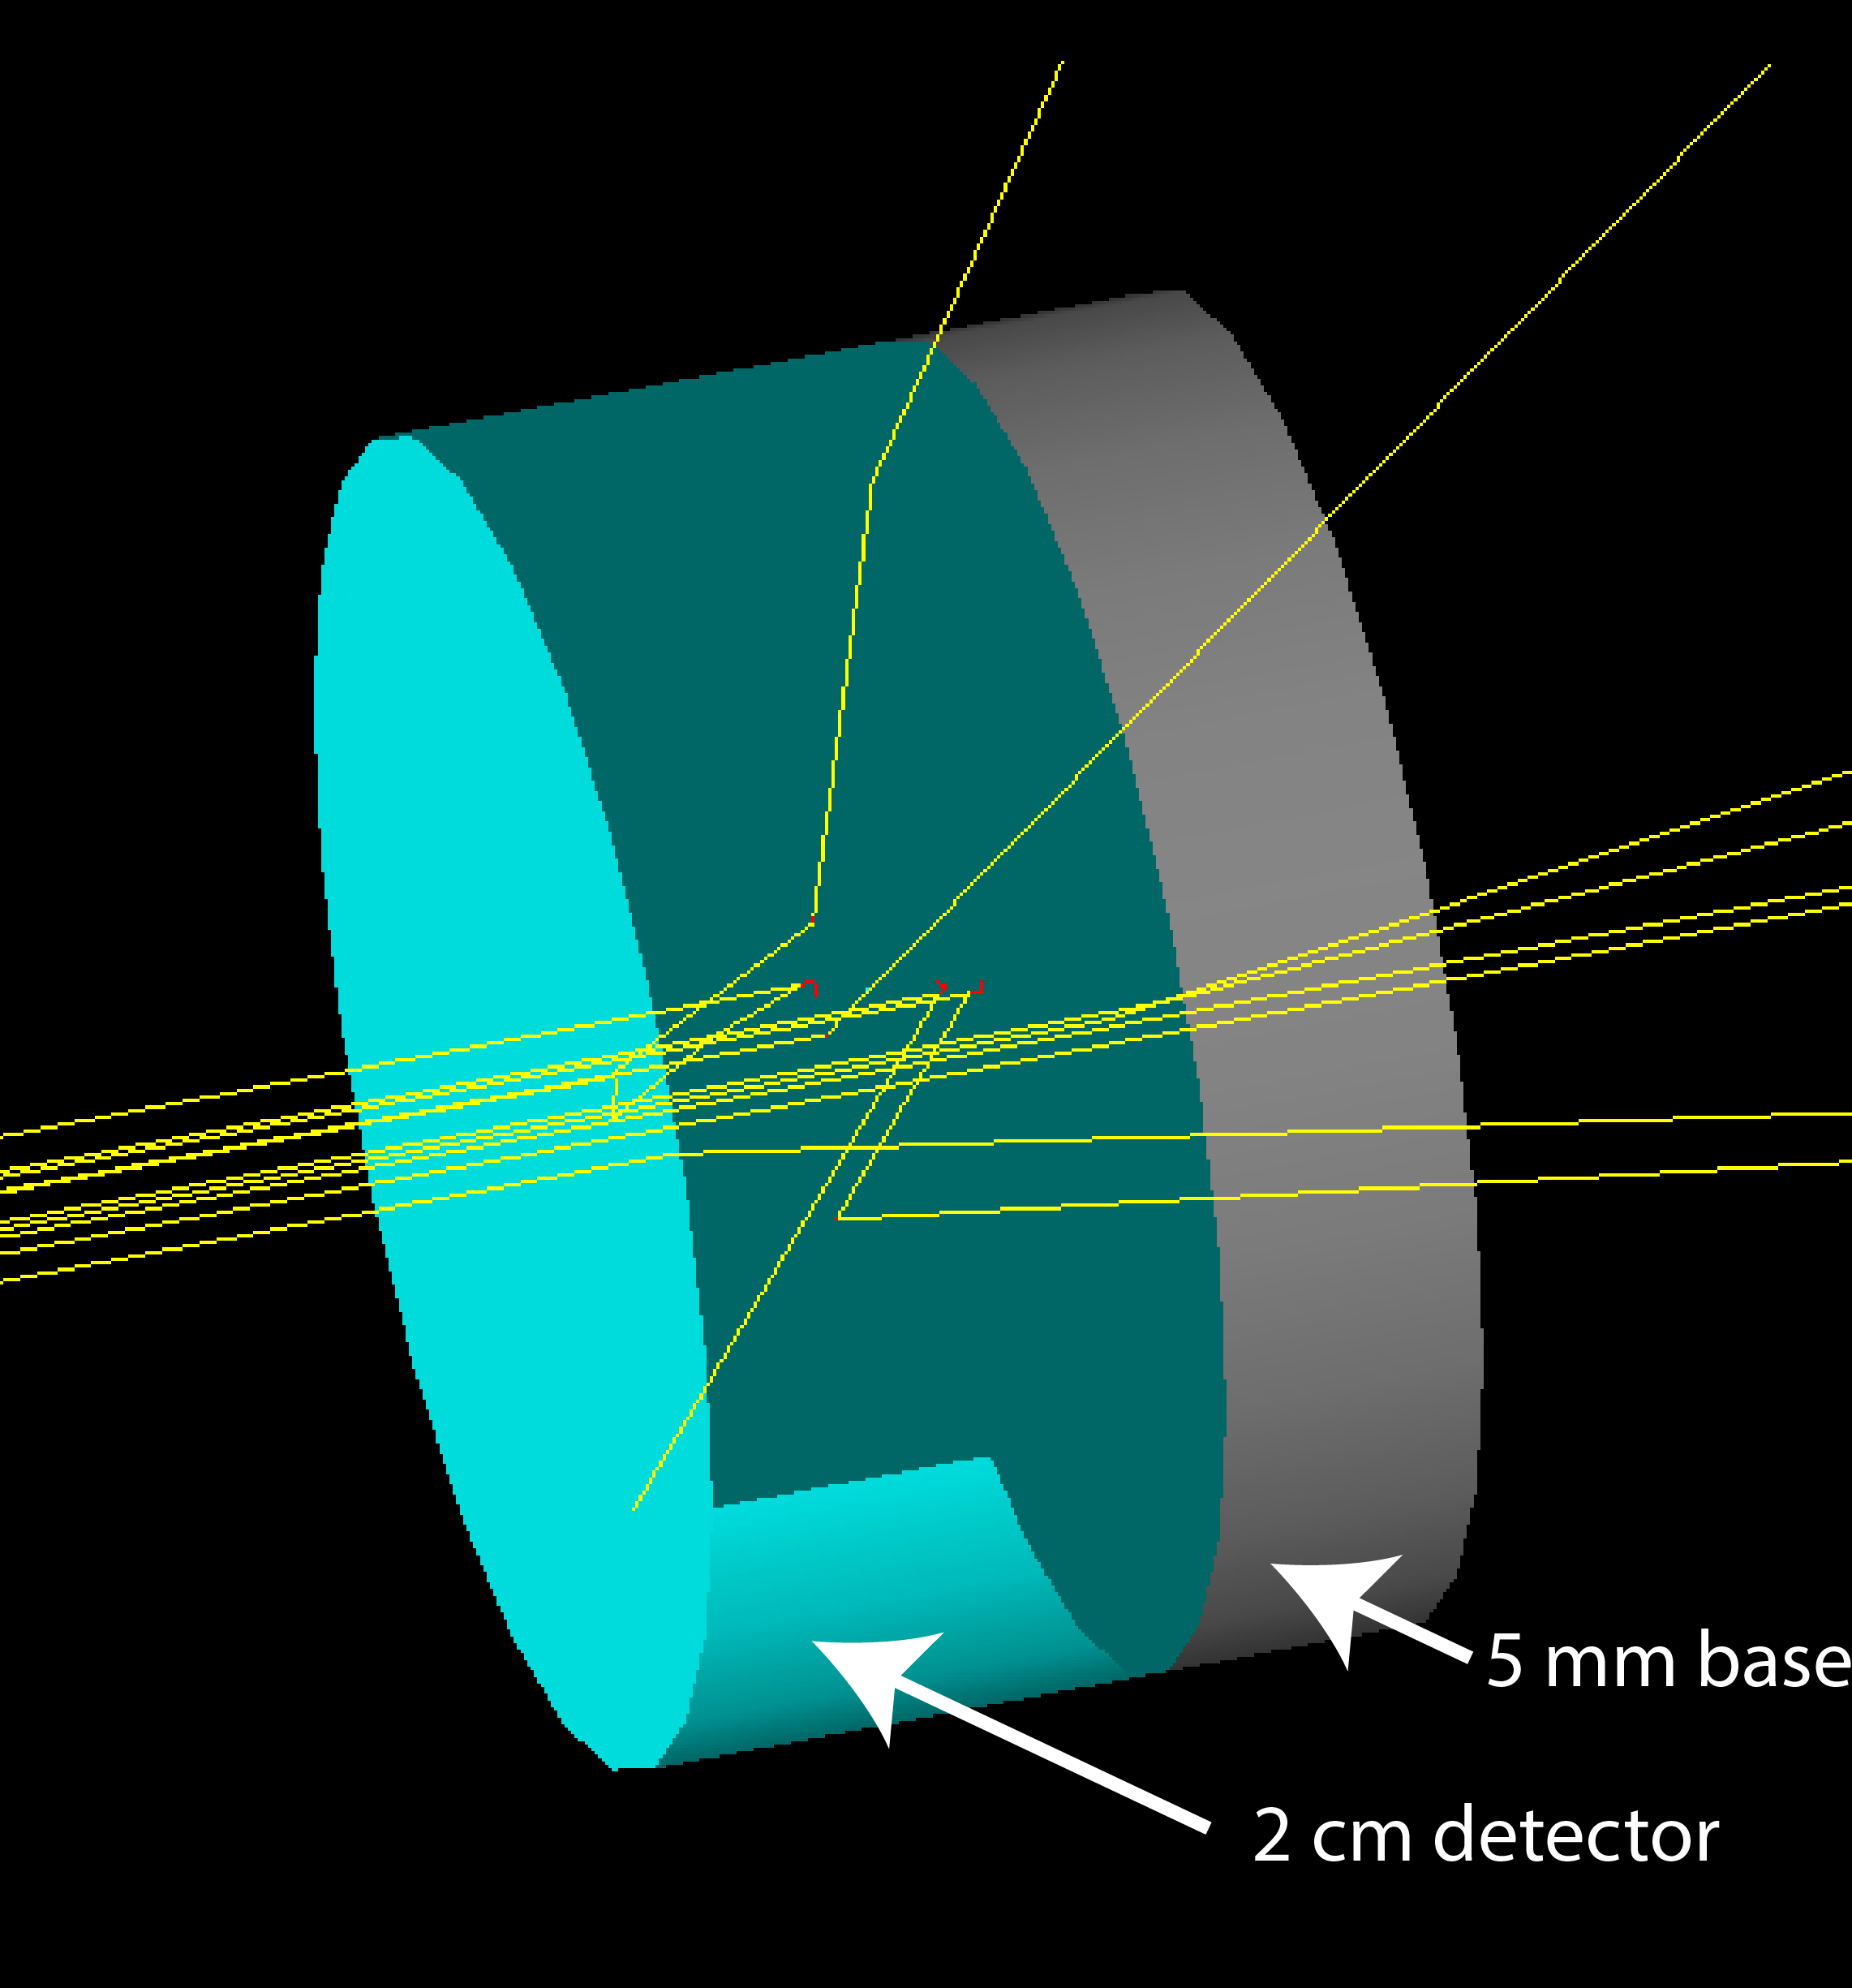
\includegraphics[width=\textwidth]{GEANT4AnnotatedGeo_EnergyDepEvent}
	\caption[GEANT4 Energy Depostion Geometry]{GEANT4 Geometry for the Simulation of Energy Deposition. What is shown are 10 photons from a \iso[60]{Co} source impigent upon a \SI{2}{\cm} thick detector.  The photon tracks are shown in yellow, while the electron tracks are shown in red.}
	\label{fig:EDepSimGeo}
\end{figure}
It is expected that the the Livermore data-driven parameterized electromagnetic physics will be necessary to calculate the ionizing energy deposition, extending the standard electro-magnetic physics down to \SI{1}{\kilo\eV}.
The neutron interactions will be simulated with a hadronic modules, using the \verb+HP+ flavored modules to use the ENDF cross sections to calculate the interaction rates.

It is proposed to validate the simulation by reproducing the single collision energy loss in water as well as comparing  the spectral shapes and averages of simulated and measured spectra.
The reproduction of the single collision energy loss will ensure that the electron physics are implemented correctly, while the simulation of the polymeric film energy deposition allows the user to gain confidence that the correct tracking and binning analysis has been implemented.




